\documentclass[
  bibliography=totoc,
  captions=tableheading,
  titlepage=firstiscover,
  twocolumn,
  %10pt,
]{scrartcl}

\setlength{\oddsidemargin}{0.0 cm}
\setlength{\evensidemargin}{0.0 cm}
\setlength{\topmargin}{-1cm}
\setlength{\textheight}{24 cm}
\setlength{\textwidth}{16 cm}

\pagestyle{plain}

\usepackage{fixltx2e}
\usepackage[aux]{rerunfilecheck}
\usepackage{polyglossia}
%\frenchspacing
\setmainlanguage[variant=british]{english}
\usepackage[intlimits]{amsmath}
\usepackage{amssymb}
\usepackage{mathtools}
\usepackage{fontspec}
\setsansfont{Helvetica}
\setmainfont{Charis SIL}
\setmonofont[Scale=0.92]{Source Code Pro}
\defaultfontfeatures{Ligatures=TeX}
\usepackage[
  math-style=ISO,
  bold-style=ISO,
  sans-style=italic,
  nabla=upright,
  partial=upright,
]{unicode-math}
\setmathfont{Tex Gyre Pagella Math}
%\setmathfont{Asana Math}
%\setmathfont{Latin Modern Math}
\setmathfont[range={\mathscr, \mathbfscr}]{XITS Math}
\setmathfont[range=\coloneq]{XITS Math}
\setmathfont[range=\propto]{XITS Math}
\removenolimits{\int}
\let\hbar\relax
\DeclareMathSymbol{\hbar}{\mathord}{AMSb}{"7E}
\DeclareMathSymbol{ℏ}{\mathord}{AMSb}{"7E}
\usepackage[autostyle]{csquotes}
\usepackage[
  locale=US,
  separate-uncertainty=true,
  per-mode=symbol-or-fraction,
]{siunitx}
\usepackage[version=3]{mhchem}
\usepackage{xfrac}
%\usepackage[section, below]{placeins}
\usepackage[
  labelfont=bf,
  font=small,
  width=0.9\textwidth,
]{caption}
\usepackage{subcaption}
\usepackage{graphicx}
\usepackage{grffile}
\usepackage{float}
\usepackage[italic]{hepnicenames}
\floatplacement{figure}{htbp}
\floatplacement{table}{htbp}
\usepackage{booktabs}
\usepackage{pdflscape}
\usepackage[
  sorting=none,
]{biblatex}
\addbibresource{main.bib}
\usepackage{microtype}
\usepackage{blindtext}
\usepackage[
  unicode,
  pdfusetitle,
  pdfcreator={},
  pdfproducer={},
]{hyperref}
\usepackage{bookmark}
\usepackage[shortcuts]{extdash}
\usepackage{tikz}
\captionsetup{width=0.45\textwidth}


\usetikzlibrary{calc}
\usetikzlibrary{arrows,shapes}

\newcommand{\package}[1]{\texttt{#1}}
\newcommand{\class}[1]{\texttt{#1}}
\newcommand{\function}[1]{\texttt{#1}}
\newcommand{\fpath}[1]{\texttt{#1}}

\captionsetup{width=0.45\textwidth}

\newcommand{\eg}{e.g.\@ }

\usepackage{hyphenat}

\begin{document}

\twocolumn[{%
\begin{center}
  {\LARGE \textbf{\textsf{Top Quark Seminar IV}}} \\
  \vspace{1em}
  {\Large \textbf{\textsf{Igor Babuschkin}}} \\
  \vspace{1em}
  {\large \textbf{\textsf{3rd November 2014}}}
\section*{Summary of \enquote{How to Combine Correlated Estimates of a Single Physical Quantity}}
\end{center}
}]

The article\cite{lyons} discusses how correlated estimates $y_i$ of a physical quantity $y$ can be combined to produce a single estimate $\hat{y}$.
Such a combination is desirable, because providing a single, clear result for a measurement allows it to be interpreted in a straightforward way.

Uncorrelated estimates can be combined by the weighted mean
\begin{equation}
  \hat{y} = \sum_i{\frac{y_i}{\sigma_i^2}} σ\:,
\end{equation}
where $σ_i$ are the errors of the individual measurements $y_i$ and $σ$ is the error of $\hat{y}$ given by
\begin{equation}
  \frac{1}{σ^2} = \frac{1}{\sum_i 1/σ_i^2 }\:.
\end{equation}

For the case of correlated estimates, the authors propose a technique called BLUE (Best Linear Unbiased Estimate).
It consists of minimizing the weighted sum of squares
\begin{equation}
  S = \sum_i \sum_j (y - y_i) (y - y_j) \mathbf{E}^{-1}_{ij}\:,
  \label{squares}
\end{equation}
where $\mathbf{E}$ is the covariance matrix of the individual estimates.
This is equivalent to determining the coefficients $α_i$ in $\hat{y} = \sum \alpha_i y_i$ through
\begin{equation}
  \mathbf{\alpha} = \frac{\mathbf{E}^{-1} \mathbf{U}}{\mathbf{U}^T \mathbf{E}^{-1} \mathbf{U}}\:,
\end{equation}
where $\mathbf{U}$ is a vector with all entries equal to one.

Taking the minimal $S$ to be $\chi^2$-distributed with $(n - 1)$ degrees of freedom allows one to judge in how far the individual measurements are compatible with each other.

The covariance matrix can be determined by providing a model that explains the correlation between the individual measurements, or approximately by performing a Monte Carlo simulation.

The authors continue by demonstrating that BLUE performs sensibly in several edge cases, for example the case of two identical, perfectly correlated measurements.
In this case, the estimate and precision of the combination correspond to those of the two individual measurements.

The authors then detail the general case of combining two correlated estimates.
An interesting effect that can occur when the two measurements are highly correlated is the occurence of negative coefficients $α_i$ in the BLUE combination, which can be seen in figure \ref{simple}.

\begin{figure}
  \centering
  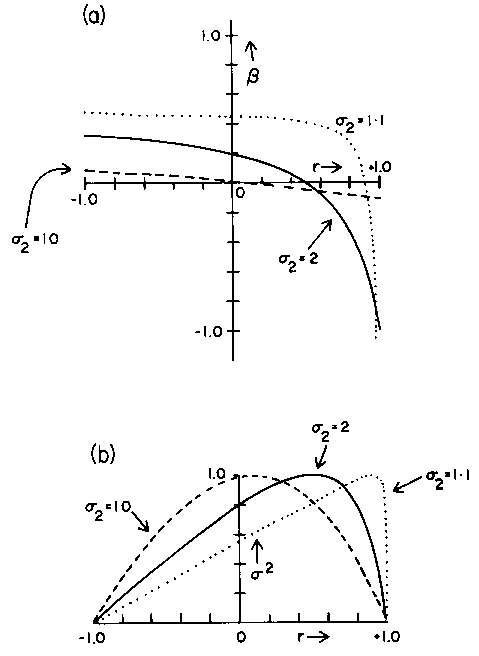
\includegraphics[width=0.45\textwidth]{./figures/simple.pdf}
  \caption{A demonstration of the combination involing two correlated values. (a) shows the size of the second combination coefficient $β$ depending on the degree of correlation $r$ between the two measurements. (b) shows the variance $σ^2$ of the final result, also depending on $r$. $σ_1$ is taken to be 1, while several possibilities for $σ_2$ are shown. \cite{lyons}}
  \label{simple}
\end{figure}

The technique is then demonstrated by applying it to a real experiment, the measurement of the charm quark lifetime at the Super Proton Synchrotron at CERN.

The charm lifetime $τ$ has been measured in four different ways\cite{augilar}: By fully reconstructing $D$ meson decays, by measuring the transverse length of decaying mesons, by measuring the impact parameter and by correcting the momentum estimate for the absence of missing decay products.

A covariance matrix for these four measurements is estimated from Monte Carlo simulation.
Because the error on as single $τ$ depends on the size of $τ$, the authors proceed to replace the individual errors on the $τ_i$ with a single error, derived from an approximation to the correct $τ$.
This is done to robustify the final estimate with regard to statistical fluctuations in the estimates $τ_i$.
The approximate choice of $τ$ is justified by the observation that the combination isn't significantly impacted by it.

The asymmetric errors of the $τ_i$ are symmetricized by taking the geometric mean.

Further, systematic errors for the four measurements are assumed to be independent, which means they can be incorporated into the estimate by modifying the diagonal of the covariance matrix.

The authors proceed to apply the BLUE method to derive a single estimate for $τ$.
They apply a $χ^2$ test to the minimal sum of squares from \eqref{squares} to check the compability of the four initial measurements and conclude that they are compatible.

The BLUE method is commonly applied in high energy physics to calculate combinations of measurements from different experiments.
One such case is the world combination of the top quark mass displayed in figure \ref{world}.
This is the first top mass combination of LHC and Tevatron results.

Monte Carlo techniques usually can't be used to derive such a combination.
Instead, different sources of uncertainty can be listed for each experiment and correlation coefficients proposed for each of them.
The correlation coefficients can be used to construct a covariance matrix.
The BLUE method can then be employed to calculate a combination.

\begin{figure}
  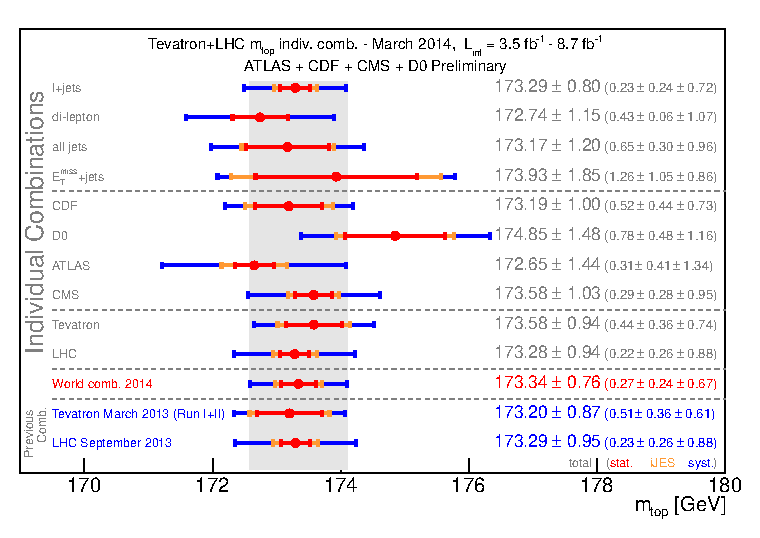
\includegraphics[width=0.5\textwidth]{./figures/world.pdf}
  \caption{World combination for the top quark mass taken from \cite{atlas}.}
  \label{world}
\end{figure}

\vspace{1em}

\nocite{*}
\printbibliography

\end{document}
